
%this was the original submission

\documentclass[letterpaper]{article}

\usepackage{natbib,alifeconf}  %% The order is important


% *****************
%  Requirements:
% *****************
%
% - All pages sized consistently at 8.5 x 11 inches (US letter size).
% - PDF length <= 8 pages for full papers, <=2 pages for extended
%    abstracts (not including citations).
% - Abstract length <= 250 words.
% - No visible crop marks.
% - Images at no greater than 300 dpi, scaled at 100%.
% - Embedded open type fonts only.
% - All layers flattened.
% - No attachments.
% - All desired links active in the files.

% Note that the PDF file must not exceed 5 MB if it is to be indexed
% by Google Scholar. Additional information about Google Scholar
% can be found here:
% http://www.google.com/intl/en/scholar/inclusion.html.


% If your system does not generate letter format documents by default,
% you can use the following workflow:
% latex example
% bibtex example
% latex example ; latex example
% dvips -o example.ps -t letterSize example.dvi
% ps2pdf example.ps example.pdf


% For pdflatex users:
% The alifeconf style file loads the "graphicx" package, and
% this may lead some users of pdflatex to experience problems.
% These can be fixed by editing the alifeconf.sty file to specify:
% \usepackage[pdftex]{graphicx}
%   instead of
% \usepackage{graphicx}.
% The PDF output generated by pdflatex should match the required
% specifications and obviously the dvips and ps2pdf steps become
% unnecessary.


% Note:  Some laser printers have a serious problem printing TeX
% output. The use of ps type I fonts should avoid this problem.


\title{An Ising-like model for language evolution}
\author{Conor Houghton \\
\mbox{}\\
Department of Computer Science, University of Bristol, UK\\
conor.houghton@bristol.ac.uk} % email of corresponding author


% For several authors from the same institution use the same number to
% refer to one address.
%
% If the names do not fit well on one line use
%         Author 1, Author 2 ... \\ {\Large\bf Author n} ...\\ ...
%
% If the title and author information do not fit in the area
% allocated, place \setlength\titlebox{<new height>} after the
% \documentclass line where <new height> is 2.25in



\begin{document}
\maketitle

\begin{abstract}
I propose a novel Ising-like model of language evolution. In a simple way, Ising-like models represent the countervailing tendencies towards stability and change present in language evolution. In the ordinary Ising-model a node on a graph, here representing a language speaker, interacts with all its neighbors. In contrast, in the model proposed in this extended abstract, a node only interacts with the neighboring node whose state-vector is most similar to its own, reflecting the tendency of people to mostly interact with others who speak a similar language to their own. Unlike the ordinary Ising model, which tends towards language continua, this model allows language boundaries. 
\end{abstract}

Languages evolve under the influence of contrary forces, forces that encourage stability and those that encourage change. For a start, languages are useful insofar as they are understood and under this imperative an individual's language should align with the languages of others. However, there is a contrary propensity towards language invention, an inclination, particularly among the young, to modify or reinvent language, either to exclude other, perhaps, older speakers or out of a simple delight in the act of language creation. Another example is found in grammar, here a move towards a more explicit and logical grammar, one that aids the speaker and listener in the precise use of language, is opposed by a sort of laziness, a desire, even at the cost of inconsistency and potential ambiguity, to employ shorter or sloppier language or to find habitual short-hand forms for frequently used expression. 

There have been useful and informative attempts to model language evolution; as an example the iterated language models simulate the emergence of compositionality in languages \cite{KirbyHurford,BraceBullock}. Here, however, my goal is it to suggest the simplest possible model that encompasses the processes of stability and change outlined above. This leads me to a simple Ising-like model. In this extended abstract I will describe the model and my motivation in proposing it. A more detailed comparison of the properties of language evolution in this model is not attempted, but I believe that this would be an interesting thing to study in future.

In an Ising model the nodes of a graph have a value of plus or minus one; because of the particular history of the Ising model this value is called the \textsl{spin} of the node. The Ising model is used to model magnetization and is important in physics because it has a phase transition and because in particular cases, one- and two-dimensional lattice graphs, it is a solvable thermodynamic model \cite{Onsager1944}. In physics the overall energy of the system is important and this energy is minimized by aligning the spins of a node with those of its neighbors in the graph. It is, however, a thermodynamic model so the nodes do not always change their states in a way that reduces this energy. In the formation that will be used here, at each time step a node is chosen and the consequence of changing its value, from plus to minus, or minus to plus, is investigated. If the current spin of the node $x$ is $s_x$ then the change to the energy that would result from flipping the sign of $s_x$ is
\begin{equation}
dE=\frac{2}{n}s_x\sum_y s_y
\end{equation}
where the sum is over all connected nodes, $n$ is the degree of the nodes, here assumed constant, and the connection strengths, the contribution of individual alignment of states to the energy has been fixed in a convenient way. If $dE$ is negative, then flipping $s_x$ lowers the energy and this change is accepted; if it is positive it is accepted with probability
\begin{equation}
    p=\exp{(-dE/T)}
\end{equation}
where $T$, the temperature, determines the magnitude of the random thermal effects. 

\begin{figure*}[ht]
\begin{center}
\begin{tabular}{lll}
\textbf{a}&\textbf{b} ordinary&\textbf{c} preference\\
\includegraphics[height=1.5in]{energy_original.png}&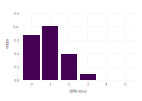
\includegraphics[height=1.5in]{ord_hist.png}&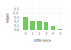
\includegraphics[height=1.5in]{evo_hist.png}
\end{tabular}
\caption{\textbf{Comparing the ordinary and preference model}. \textbf{a} plots the energy per spin as a function of temperature; the simulation is run for a $50\times 50$ periodic grid and finite size effects smooth the phase transition in the ordinary model, it is nonetheless visible at around $T=0.28$. This is only different from the standard critical temperature because of the choice made in the connection strength. For the preference model, there also appears to be a change in behavior at the same temperature, though the change is more gradual. \textbf{b} and \textbf{c} plot the similarity of nodes each side of an edge; for each edge the Hamming difference between the states is histogrammed and normalized to give a probability. It shows the difference between the two models, with the preference model allowing neighboring nodes to differ considerably more. For all three plots the average result of ten trials is shown and for each trial the model is run for 25,000 time steps to allow it to reach equilibrium.}
\label{figure}
\end{center}
\end{figure*}

In this way, the Ising model models the key aspect of language evolution noted above: there is a competition between alignment and randomness and so the simplest putative Ising-like model of language evolution would simply be an Ising model on a two-dimensional square lattice, the lattice representing the geographical distribution of speakers. However, this would only allow for two languages, the ``up-language'' and the ``down-language''. To address this shortcoming, the individual spin $s_x$ is replaced with a vector of spins $\textbf{s}_x$ which will be referred to as the state of the node; the idea is that each of the individual spins corresponds to a property of the language, so, for example one spin in $\textbf{s}_x$ might be thought of as determining the order of noun and adjective. In this model, a node is chosen at random and for that node one component of the state vector is selected, again randomly. This component is flipped, or left unflipped, using the same thermodynamics as described above. If the state vector has length $L$ this model of language evolution is, effectively, $L$ independent Ising models. It would be possible to compare this model to the distribution of languages, attempting to use the distribution of cluster sizes for example, to fix a value of the temperature $T$ and state size $L$. Something of this sort is done using a slightly different model in \cite{SivaEtAl2015,SivaEtAl2017} with interesting result.

There is an  problem with this model. Famously a putative nineteenth century traveler could walk from Lisbon to Naples without ever crossing a language boundary; although Portuguese and Neapolitan are very different languages, people living near each other are always able to communicate. This is a property of the $L$-state Ising model. However, in the real world, language continua are common but not universal, if the putative traveler varied their route just a small bit they would pass through the Basque country and in doing so, they would certainly cross a language boundary. To explain this, I note, crucially, when learning a language an infant does not poll its neighbors and use a mixture as an exemplar; it typically learns from people in its household, often parents, and after that will preferential communicate with other people who speak a language similar to theirs. Here, I am proposing that this be incorporated into our simple model of language evolution, somewhat in the spirit of the bounded confidence model \cite{HegselmannKrause2019}.

I will call this model the \textsl{preferential model} and the original $L$-state Ising model, the \textsl{ordinary model}. In the preferential model, at each time step, a node is, again, chosen at random and, again, a component of the state vector is selected. Now, however, the Hamming distance is calculated between the state vector of the node and the state vector for its four neighbors and the closest neighbor is chosen, this might involve a random selection if there are equally close nodes. The same thermodynamical calculation, with $n$ now set to one, determines whether or not to flip the spin. In this preferential model there is a mixture of language continua and language boundaries. This is illustrated in Fig.~\ref{figure}. 

I suggest that the preferential model is the simplest model of language evolution to capture its the two key properties of stability and change. There are lots of potential variations of the model such as local temperature changes, weighted random selection of the preferred neighbor and interaction between components of the state vector. However, before consider further variants, the properties of the current model should be studied: what is the nature, for example, of the transition around the temperature where the ordinary model has its phase transition; how does the model change as the length of the state vector is varied, are there other variants in which the state spins are coupled. The model also needs to compared to language data to decide if this simple model has any potential to describe, in a meaningful and interesting way, the distribution of languages. 

\section{Code availability}
Code will be made available when the paper is de-anonymised.
\section{Acknowledgements}
Colleagues and funders  will be acknowledged when the paper is de-anonymised.
\newpage
\footnotesize
\bibliographystyle{apalike}
\bibliography{bibliography} % replace by the name of your .bib file


\end{document}
